\section{Kernel methods}

%% Linear classification {{{
\subsection{Linear classification}

At first, we create three datasets, with different distances between
the means of two classes, so that there is one with no overlap,
one with heavy overlap and one semi-overlapping.
Each dataset consists of the coordinates of the points $\v{x}_i\in\mathbb{R}^2$,
and the corresponding classification $y_i\in\{-1, 1\}$.

Three classifiers are implemented.

\subsubsection*{Soft Margin Support Vector Classification}

% With the original SVC, we are looking for the parameters of the affine function
% that best separates the two classes: $\sum\limits_{i=1}^ny_i\brc{w\T\,x_ib}=0$.
% This way, the separating line is going to be halfway between two specific
% points of the two classes. The distance between the line and these vectors
% has to be maximized, and that is done by minimizing $w$.
% However, this can only be done on linearly separable datasets,
% so a different solution is needed.

The support vector classifier is a modification of Vapnik's SVC, such that
badly classified data points are penalized.

The problem can be solved via convex optimization, using the cvxpy python library.
\begin{equation}
\begin{split}
	&\underset{\v{w},\,\epsilon\in\mathbb{R}^d,\,b\in\mathbb{R}}{\operatorname{minimize}}\HS
		\frac{1}{2}\,\norm{\v{w}}^2 + \lambda\,\sum\epsilon\\
	&\text{subject to}\HS
		y_k\,\brc{\v{w}\T\,\v{x}_k + b}\geq1-\epsilon_k\hs\text{and}\hs\epsilon_k\geq0\HS\text{for}\hs k=1,\dots n
\end{split}
\end{equation}

\subsubsection*{Least Squares SVM}

LS-SVM is the least squares reformulation of Vapnik's SVC.
This too can be solved via convex optimization.
\begin{equation}
\begin{split}
	&\underset{w,\,\epsilon\in\mathbb{R}^d,\,b\in\mathbb{R}}{\operatorname{minimize}}\HS
		\frac{1}{2}\,\norm{\v{w}}^2 + \lambda\,\sum\epsilon^2\\
	&\text{subject to}\HS
		y_k\,\brc{\v{w}\T\,\v{x}_k + b} = 1-\epsilon_k\HS\text{for}\hs k=1,\dots n
\end{split}
\end{equation}

\subsubsection*{Nearest centroid classifier}

With the NNC solution, the means of the classes are calculated.
Now a new sample would be classified in the class whose mean
it is closer to.

The plots of the classifiers applied to the different datasets
can be seen on figure \ref{fig:linear-classification}.

\begin{figure}[H]
	\centering
	\begin{subfigure}{\textwidth}
		\centering
		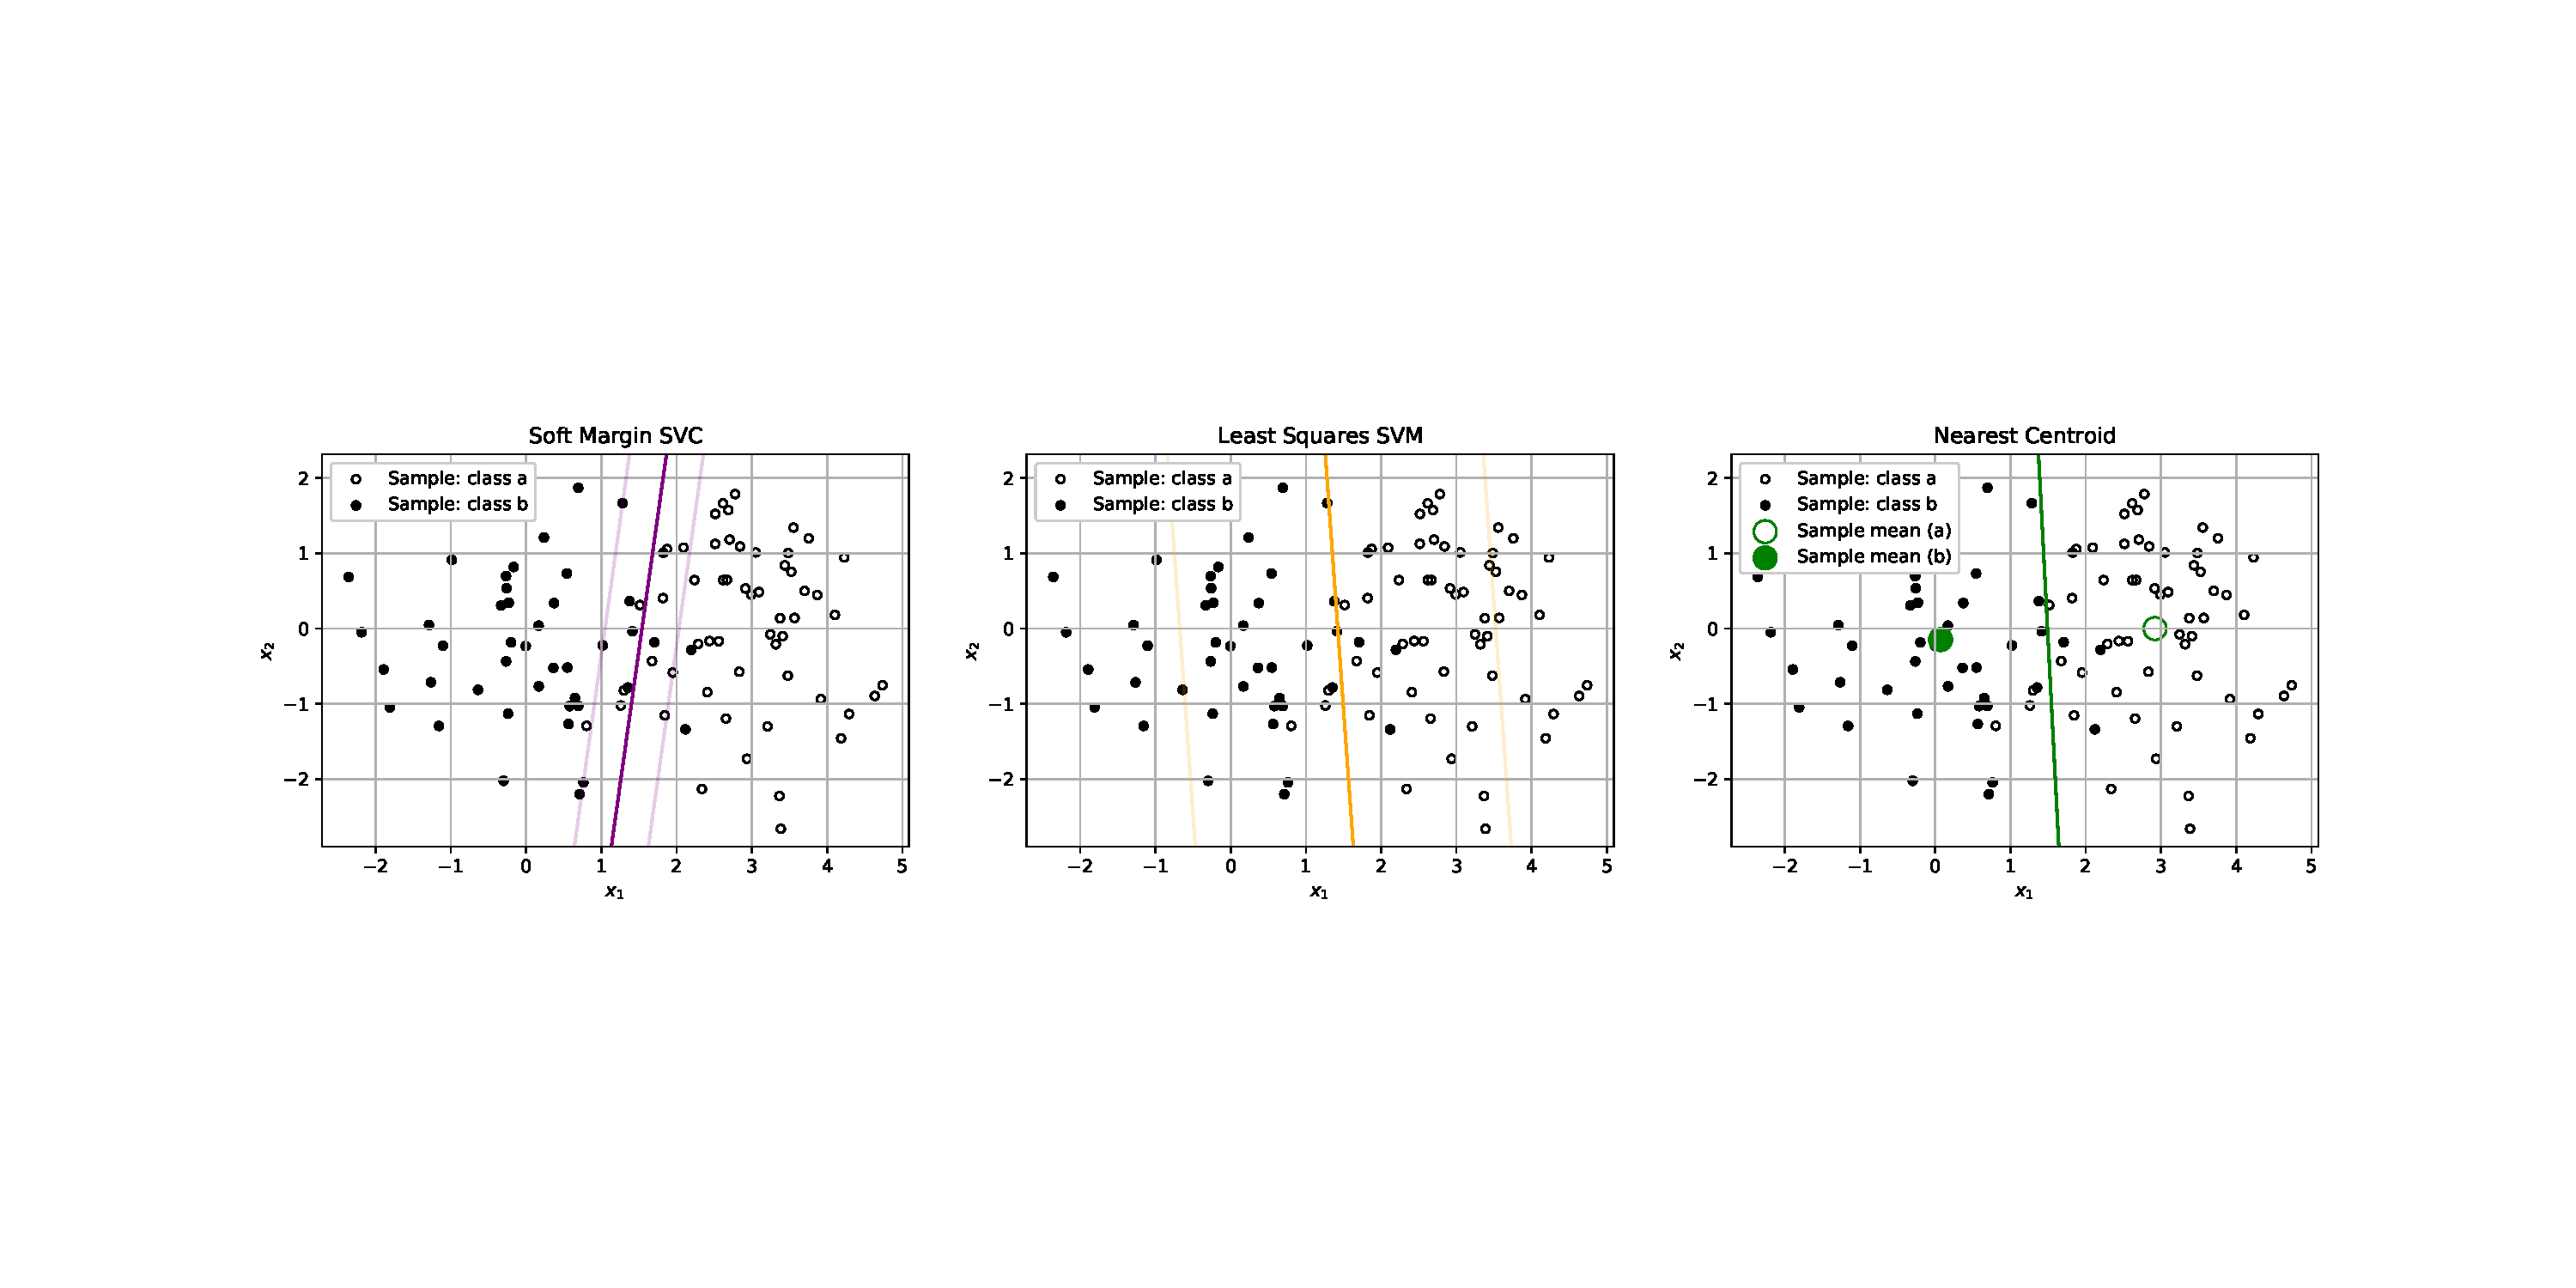
\includegraphics[width=\textwidth, trim={5cm, 7cm, 5cm, 8cm}, clip]{ex_II_1_plots_0}
		\caption{Heavily overlapping distributions}
	\end{subfigure}
	\begin{subfigure}{\textwidth}
		\centering
		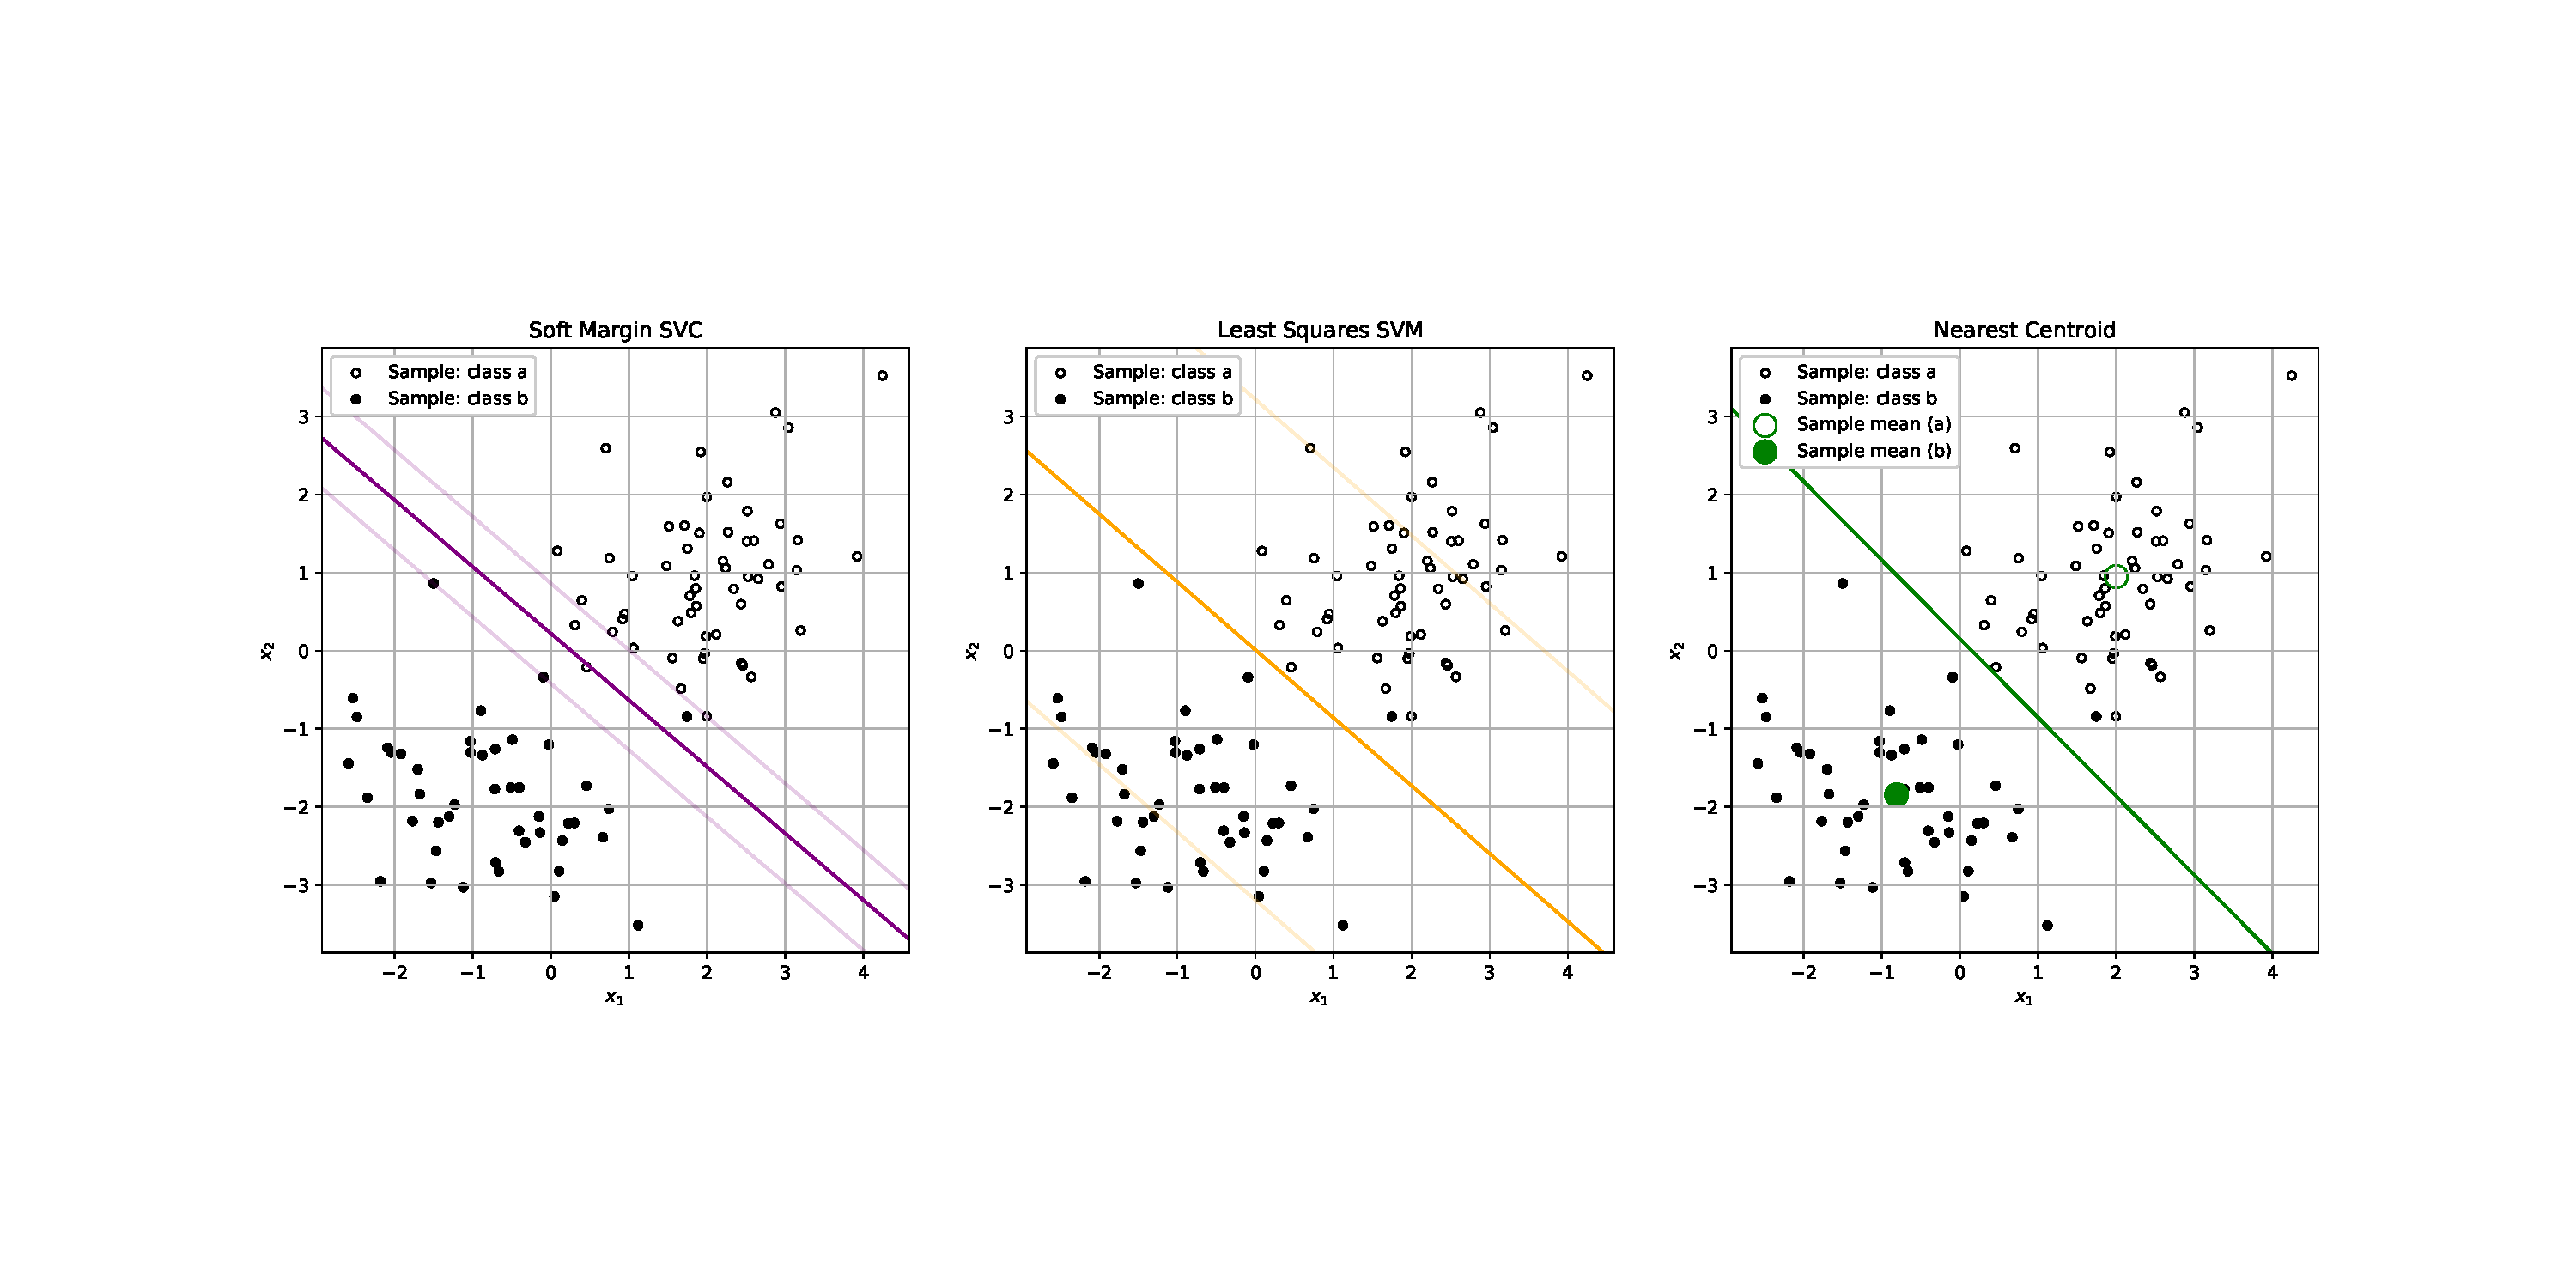
\includegraphics[width=\textwidth, trim={5cm, 5cm, 5cm, 6cm}, clip]{ex_II_1_plots_1}
		\caption{Semi-overlapping distributions}
	\end{subfigure}
	\begin{subfigure}{\textwidth}
		\centering
		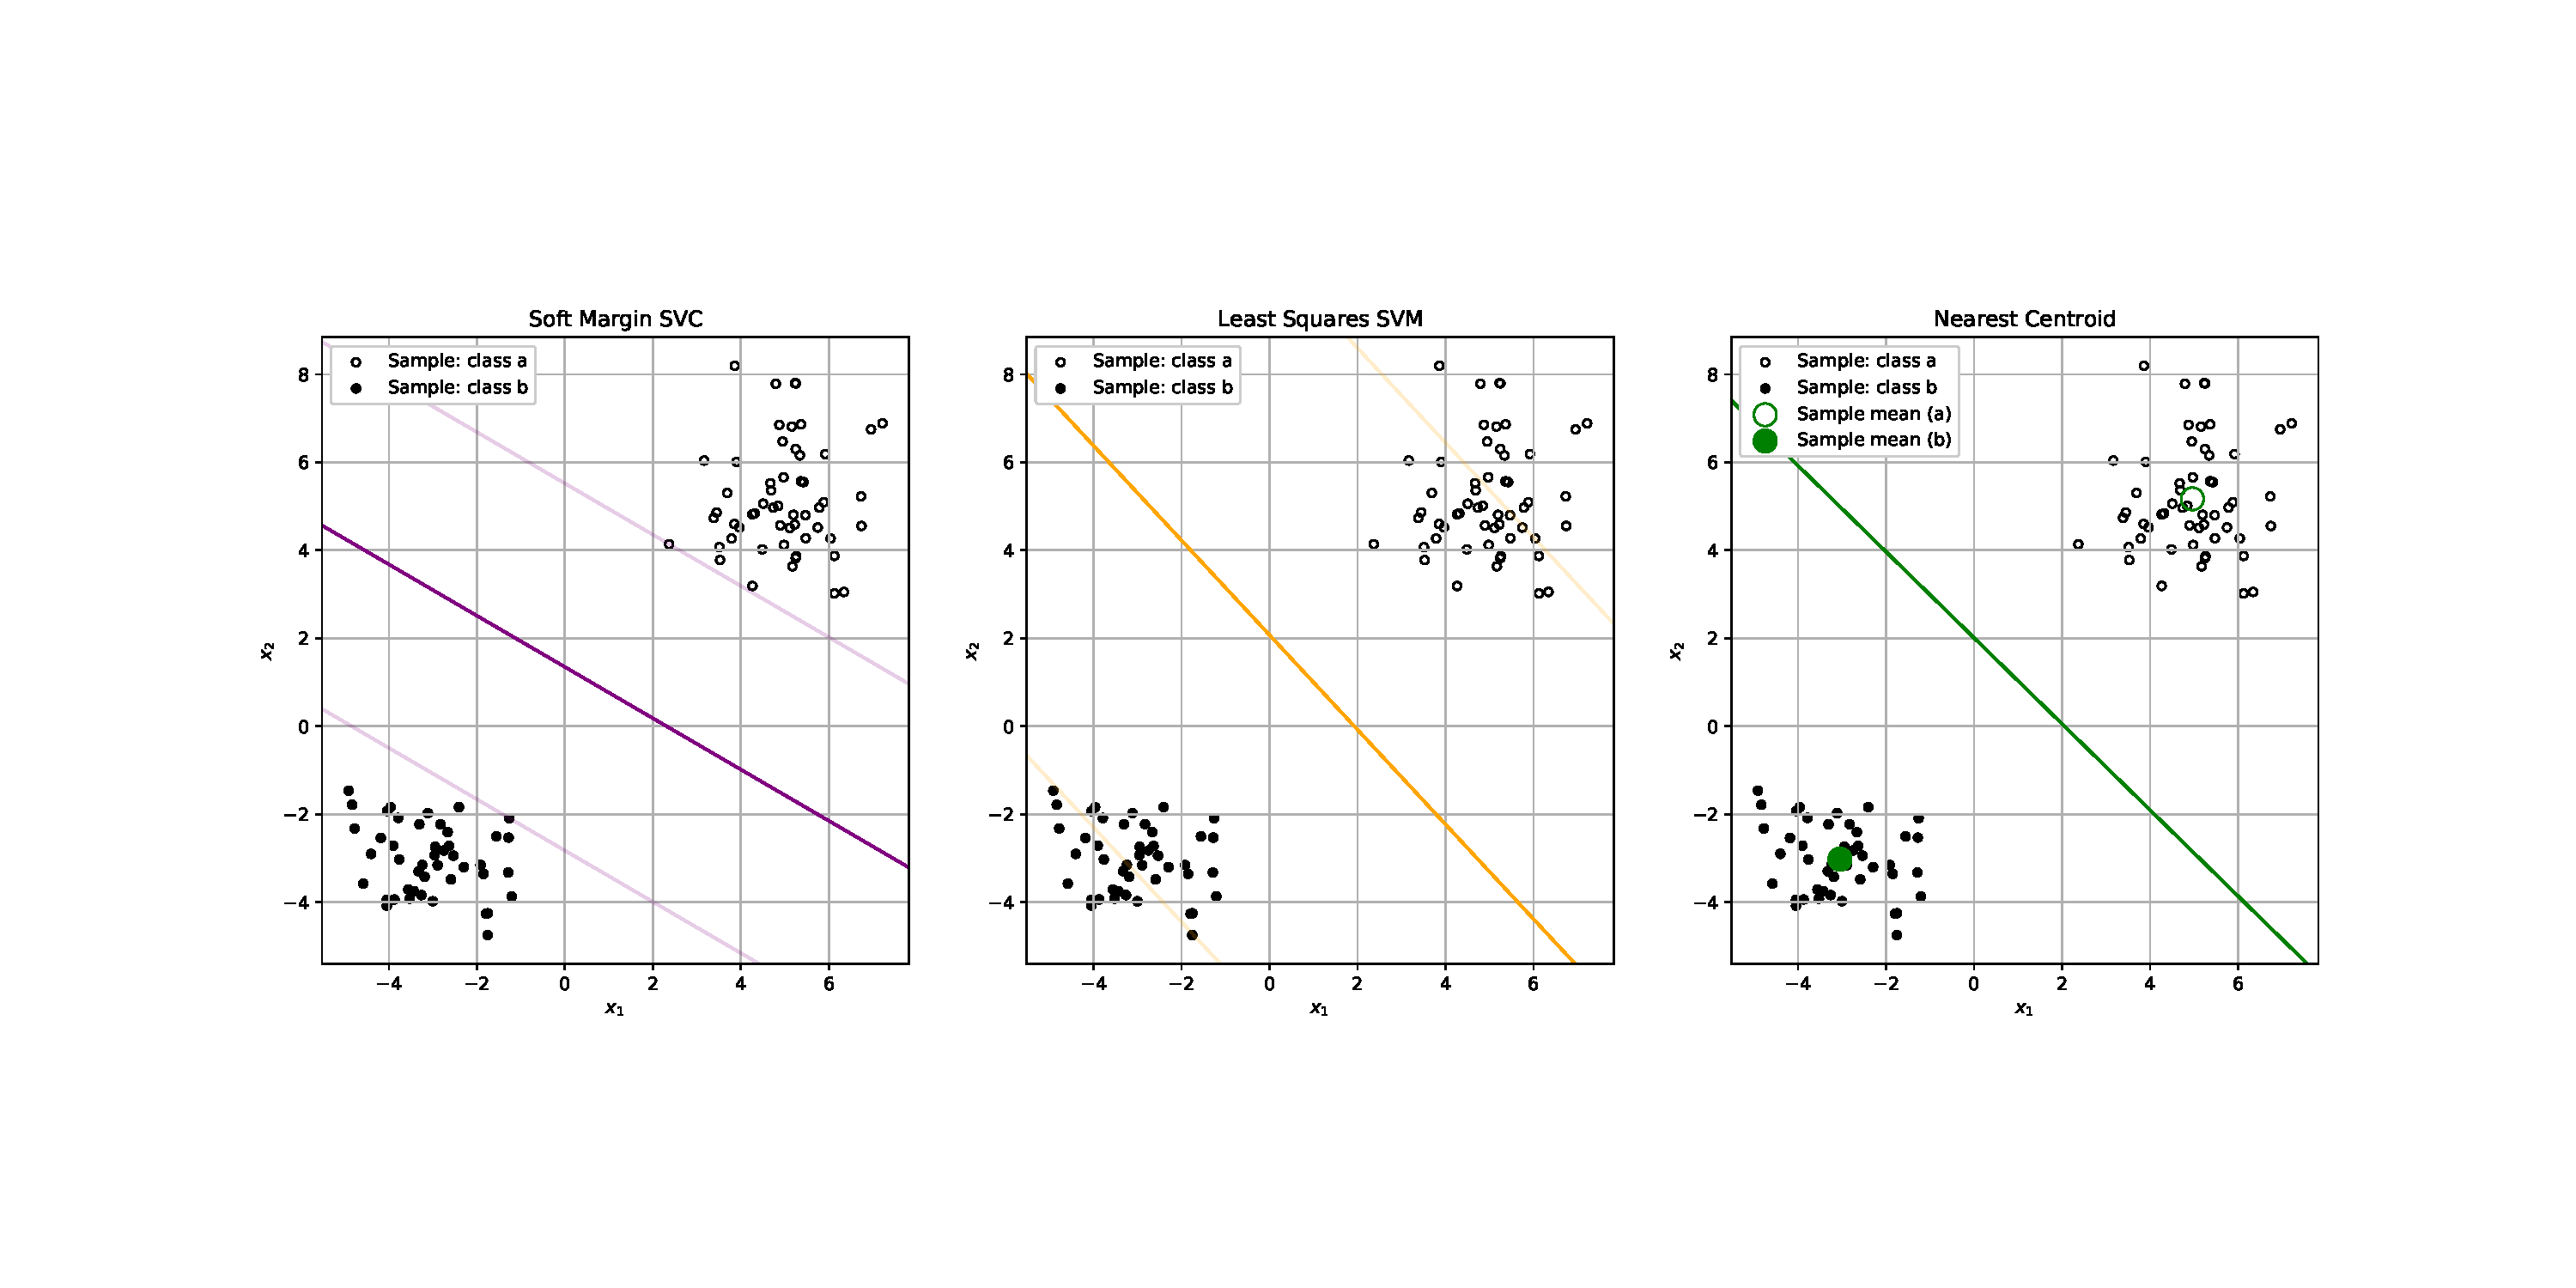
\includegraphics[width=\textwidth, trim={5cm, 5cm, 5cm, 6cm}, clip]{ex_II_1_plots_2}
		\caption{Non-overlapping distributions}
	\end{subfigure}
	\caption{Linear classification experiments}
	\label{fig:linear-classification}
\end{figure}

%% }}}

%% Nonlinear classification {{{
\subsection{Nonlinear classification}

In the next exercise a linearly not separable problem is going to be solved
via the kernelized soft margin SVC.

At first, a dataset is generated much like before, except that one of them concentrically
surrounds the other. For this to be solved via an SVC, the points need to be mapped
to a Reproducing Kernel Hilbert Space, called the feature space.
This is done with the Gaussian kernel:
\begin{equation}
	\fn{k}(\v{x}, \v{y}) = \exp\frac{-\norm{\v{x}-\v{y}}^2}{\sigma^2}.
\end{equation}
Then we define matrix $\v{K}$ as $\v{K}_{ij} = \fn{k}(\v{x}_i, \v{x}_j)$.

This poses a convex optimization problem, the dual of which is going to be solved:
\begin{equation}
\begin{split}
	&\underset{\alpha\in\mathbb{R}^n}{\operatorname{maximize}}\HS
		% \sum\limits_{k=1}^n\alpha_k - \frac{1}{2}\,\sum\limits_{k=1}^n\sum\limits_{m=1}^n\alpha_k\,\alpha_m\,y_k\,y_m\,k(x_k, x_m)\\
		\sum\limits_{k=1}^n\alpha_k - \frac{1}{2}\,(\v{\alpha}\odot\v{y})\T\v{K}(\v{\alpha}\odot\v{y})\\
	&\text{subject to}\HS
		\sum\limits_{k=1}^n\alpha_k\,y_k=0\hs\text{and}\hs\lambda\geq\alpha_k\geq0\HS\text{for}\hs k=1,\dots n,
\end{split}
\end{equation}
where $\odot$ indicates elementwise multiplication.
This ensures sparsity, specifically, for every $\alpha_k\neq0$, $x_k$ is a support vector.
$b^*$ can be calculated from KKT.

From this, the classifier function is the following:
\begin{equation}
	\fn{f}(\v{x}) = \operatorname{sign}\left[\sum\limits_{k=1}^n\alpha_k^*\,y_k\fn{k}(\v{x}, \v{x}_k) + b^*\right]
\end{equation}

The dataset along with the classification boundaries is shown on figure \ref{fig:kernel-SVC}.

\begin{figure}[H]
	\centering
	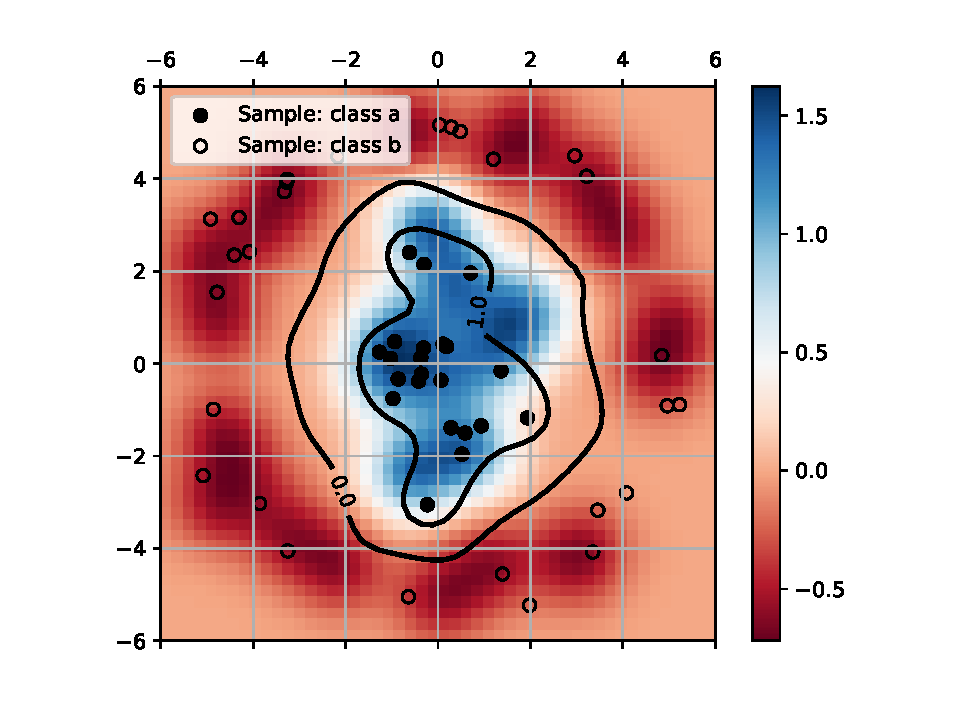
\includegraphics[width=.5\textwidth, trim={2cm, 1cm, 2cm, 5mm}, clip]{ex_II_2_plots_1}
	\caption{Nonlinear classification}
	\label{fig:kernel-SVC}
\end{figure}

%% }}}
